% ------- Create Preamble ------------
\documentclass[12pt]{article}
\usepackage[a4paper]{geometry} 
\usepackage{amsmath, amsthm, amssymb, amsfonts}
\usepackage{graphicx,epsfig}
\usepackage{booktabs} 
\usepackage{pslatex} 
\usepackage{caption} 
\usepackage{setspace} 
\usepackage{hyperref}
\usepackage{cleveref}
\usepackage{multicol, multirow}
\usepackage{graphicx,epsfig}
\usepackage{booktabs}
\usepackage{pslatex}
\usepackage{caption}
\usepackage{setspace}
\usepackage{hyperref}
\usepackage{multicol}
\usepackage{textgreek}
\usepackage{pdfpages}
\usepackage{longtable}
\usepackage{float}
\usepackage{natbib} % For references
\bibpunct{(}{)}{;}{a}{}{,} % Reference punctuation
\def\citeapos#1{\citeauthor{#1}'s (\citeyear{#1})}
\newtheorem{hypothesis}{Hypothesis}
\newtheorem{nullhypothesis}{Null Hypothesis}
\usepackage{xcolor}
\hypersetup{
    colorlinks,
    linkcolor={blue!50!blue},
    citecolor={blue!50!blue},
    urlcolor={blue!80!blue}
}
\usepackage{arydshln}
%---Set up author and title page
\singlespace
\title{Changing Norms and Partisan Polarization: How elites advance mass polarization \\\large \textit{A Pre-Analysis Plan}}
\author{Damon C.\ Roberts\footnote{PhD Candidate,
Department of Political Science, University of Colorado Boulder, UCB 333, Boulder, CO 80309-0333. Damon.Roberts-1@colorado.edu.\newline Code for replicating design declarations and diagnoses can be found at \url{{https://github.com/DamonCharlesRoberts/elite_norms_mass_polarization}}}}

%set up document
\date{\today}
\begin{document}
\maketitle
\begin{abstract}
The American public are polarized. There is debate among scholars, however, as to where this polarization comes from. Some argue that polarization is the result of growing differences in policy preferences, and others argue that it is the result of strengthening and more distinguishable identities. For those making the argument that polarization is the result of identity, it remains unclear where resulting identity-based behaviors come from. This project argues that the public learn polarizing behavior from the norms of how to participate in politics from polarized politicians. Further, it argues that popular measures of affective polarization contain this performative adherence to norms by those wanting to be ``good partisans". The present manuscript proposes three studies to examine this question. The first examines whether the public have the capacity to detect such differencing behavior. The second and third studies examine whether they punish co-and-out-partisans for engaging in this differencing behavior and whether exposure to such elite behavior encourages subjects to report higher levels of affective polarization as measured by differences in affinity towards the parties. 
\end{abstract}

\newpage 
\section{Summary of project}
While many agree that political polarization characterize contemporary American politics, scholars are somewhat divided over questions of why the public are polarized. Some argue that political polarization is guided by positive or negative emotional attachments members of the public have toward their party \citep[see][]{iyengar_et-al_2012} with which they see as a social identity. Others argue that polarization is the result of division over ideological differences \citep[see][]{fiorina_abrams_2008}.

Taking the first position as true, we should expect that, as a social identity, there are expecations about group membership due to the definitions which provide differentiation between these groups \citep{huddy_2001}. One way this is done is through norms which provide information to members of the group about what behavior is appropriate in reference to those behaviors directed toward members of the in-group and out-group. For partisans, scholars have detected a number of behaviors indicating discrimmination toward out-partisans and preferences for co-partisans \citep[see][]{iyengar_westwood_2015}.

The extant literature provides no clear direction as to whether these behaviors are learned or natural. As we hold a number of social identities with different meanings and can do so simultaneously, what appears most reasonable is that these norms of behavior for this particular partisan identity are learned. As the public rely on heuristics to process political information \citep{converse_1964}, they often rely on information from professional observers of politics and most importantly from political elites \citep{zaller_1992}.This means that one potential source of information about how to behave around co-and-out-partisans comes from members of the public watching what politicans do with co-and-out-partisan colleagues. As individuals are often motivated through group-justification, we should expect that when the public see political elites engage in such behavior, the public will want to follow suit to demonstrate solidarity with the group \citep{jost_et-al_2022_n}. This comports with evidence suggesting that political polarization in the public is expressive \citep{huddy_et-al_2015_apsr, pickup_et-al_2020}.

Polarization among elites do not appear to be all that different than in the public. Political scientists have moved passed the idea that political elites are only ideologically polarized and provide evidence which suggests that they are just, if not more, affectively polarized than the public \citep{enders_2021}. Documentation of this affective polarization comes from more than self-reported surveys like we get from the public, but also through efforts such as detecting the frequency by which members of congress interact with in-and-out-partisans on the floor of the U.S. House of Representatives between between votes \citep{dietrich_2021}. That is, one can watch the news and see the presence of polarization.

These behavioral manifestations of affective polarization may be a choice that politicians make to symbolically make a statement about their loyalty to co-partisan colleagues and to their electoral base. This potentially is a source of information for voters. This information is rather easy to process and interpret, void of complex technical details about policy and issues, and provides useful information about what is expected of them as a member in possession of a particular partisan affiliation.

If this mechanism is indeed what explains the presence of affective polarization among the public, not only does this have implications for our understanding of incentives for political elites and to clarify the seemingly endogenous relationship between polarization in the public and among elites, but it also has implications for current pouplar measures. Current measures of affective polarization in surveys utilize feeling thermometer scales where respondents are asked to rate each party on a scale running from 0 - 100 with 0 representing ``coldness" felt towards that party or 100 with ``warmness" felt towards the party. The difference between the reported feeling of warmth or coldness of the two parties represents the degree to which that person holds affectively polarized views. While these measures express valence and the degree to which it is present\footnote{Though, there are some who are quite critical of these measures' ability to capture affective polarization either as an issue of the scale or conceptually \citep[see][]{druckman_levendusky_2019}.}, the measure may additionally capture the \textit{desire} to show distance between the two parties. That is, part of the differences in these feeling thermometer scores may be partially performative as they are emulating co-partisan elites engage in similarly exaggerated differentiation between them with out-partisans. If true, this has implications for the way we think about the measure.

I propose the three following studies to investigate the following hypotheses: \textbf{$H_1$}: The public recognize and can detect behavioral differences between the way co-partisan and out-partisan elites interact with their colleagues.
\textbf{$H_2$}: As they can recognize these behavioral norms about appropriate behavior with co-and-out-partisans, the public punish co-partisans who do not take steps to differentiate themselves from out-partisans and will punish out-partisans for engaging in such differentiating behaviors. Likewise, the public will reward co-partisans who do take steps to differentiate themselves from out-partisans and will also reward out-partisans who take fewer steps to differentiate themselves from the respondent's party.
\textbf{$H_3$}: Respondents who are primed to think about their partisan identity will have exaggerated differences in feeling thermometer scores of the two parties and will also refer to themselves as stronger partisans than those who do not have the same prime. 

\section{Description of Studies}
For the experimental studies, I follow the Model-Inquiry-Data Strategy-Answer Strategy (MIDA) procedure outlined by \citet{blair_et-al_2019}. As opposed to using power analyses where all other features are considered to be optimal, the MIDA procedure allows for comparisons of design performance with simulations where various features from model choice and estimator, design and sampling choices, and the estimand are all explicitly specified. Following processes such as these reduce the chances of p-hacking through requiring researchers to be clear about their research design choices before seeing the data or running preliminary models \citep{brodeur_et-al_2022_wp}.

As there are a total of three studies the total number of participants across the three experimental studies should be no more than $1500$ individuals. The studies will be from the same sample and will recieve the same treatment. Distinguishing them as three separate studies serves the purpose of making clear the outcome of interest. The figures representing the diagnoses of the estimators explicitly define how large the proposed sample size is for the given study. So long as the statistical power stays above $0.8$, we are at the standard - where we should expect that, on average, $1$ out of $5$ times we commit Type II error.

$\text{treatment}_i$ in all of these studies refers to subjects' exposure to information suggesting this differencing behavior by elites. The treatment will take the form of a text-based vignette which provides a brief news report about a recent vote on a high-use interstate highway funding bill. Though this is not a visual treatment manifesting differencing behavior, text-based information expressing group differences are relatively common. In a recent study examining the behavior of members of Congress on twitter estimate that just under $20\%$ of tweets contain rhetoric expressing group differences based on partisanship \citep{ballard_et-al_2022_lsq}. When considering that not all politicians take on this ``legislative style" as some prefer to share messages that communicate directly to constituents about what they are doing for them \citep{bernhard_sulkin_2018}, Text-based treatments also are relatively easier to maintain internal validity than image-based information as manipulation of images might be flawed and highly suspect as original or due to a lack of equivalency between treatments when using different images between conditions.

\subsection{Study 1}
To test $H_1$, the outcome of interest is whether individuals are able to detect behavioral differences among elites with regard to how they treat out-partisan colleagues. From the discussion above, the data generating process under randomization is expected to be: 
\begin{equation}
\begin{aligned}
\text{Detection}_i = \text{treatment}_i +  + \\ 
     \text{treatment}_i \times \text{partisan congruence}_i + \\ + \epsilon_i
\end{aligned}
\label{eq:study1}
\end{equation}

%I specify OLS as the estimator for both designs which include the relevant controls, and interaction terms. For the two-arm design, the interaction comes from a question prompting the participant to report the amount of news they consume. In this design, the respondent is randomly assigned into the treatment or control condition as they traditionally would be in a two-arm design. In the block design, participants are asked the extent to which they consume the news and are placed into a ``below average" or an ``above average" block. Within each block, respondents are randomly assigned into either the control or treatment condition. The interaction term in the model for the block design comes from the binary coding of which block the respondent was placed into.

%After conducting simulations of such designs and modeling strategies, across varying effect sizes, between $-0.5$ and $0.5$, \Cref{fig:study1} presents the bias, RMSE, and statistical power resulting from these designs and estimators given the data generating process described above.

%\begin{figure}
%     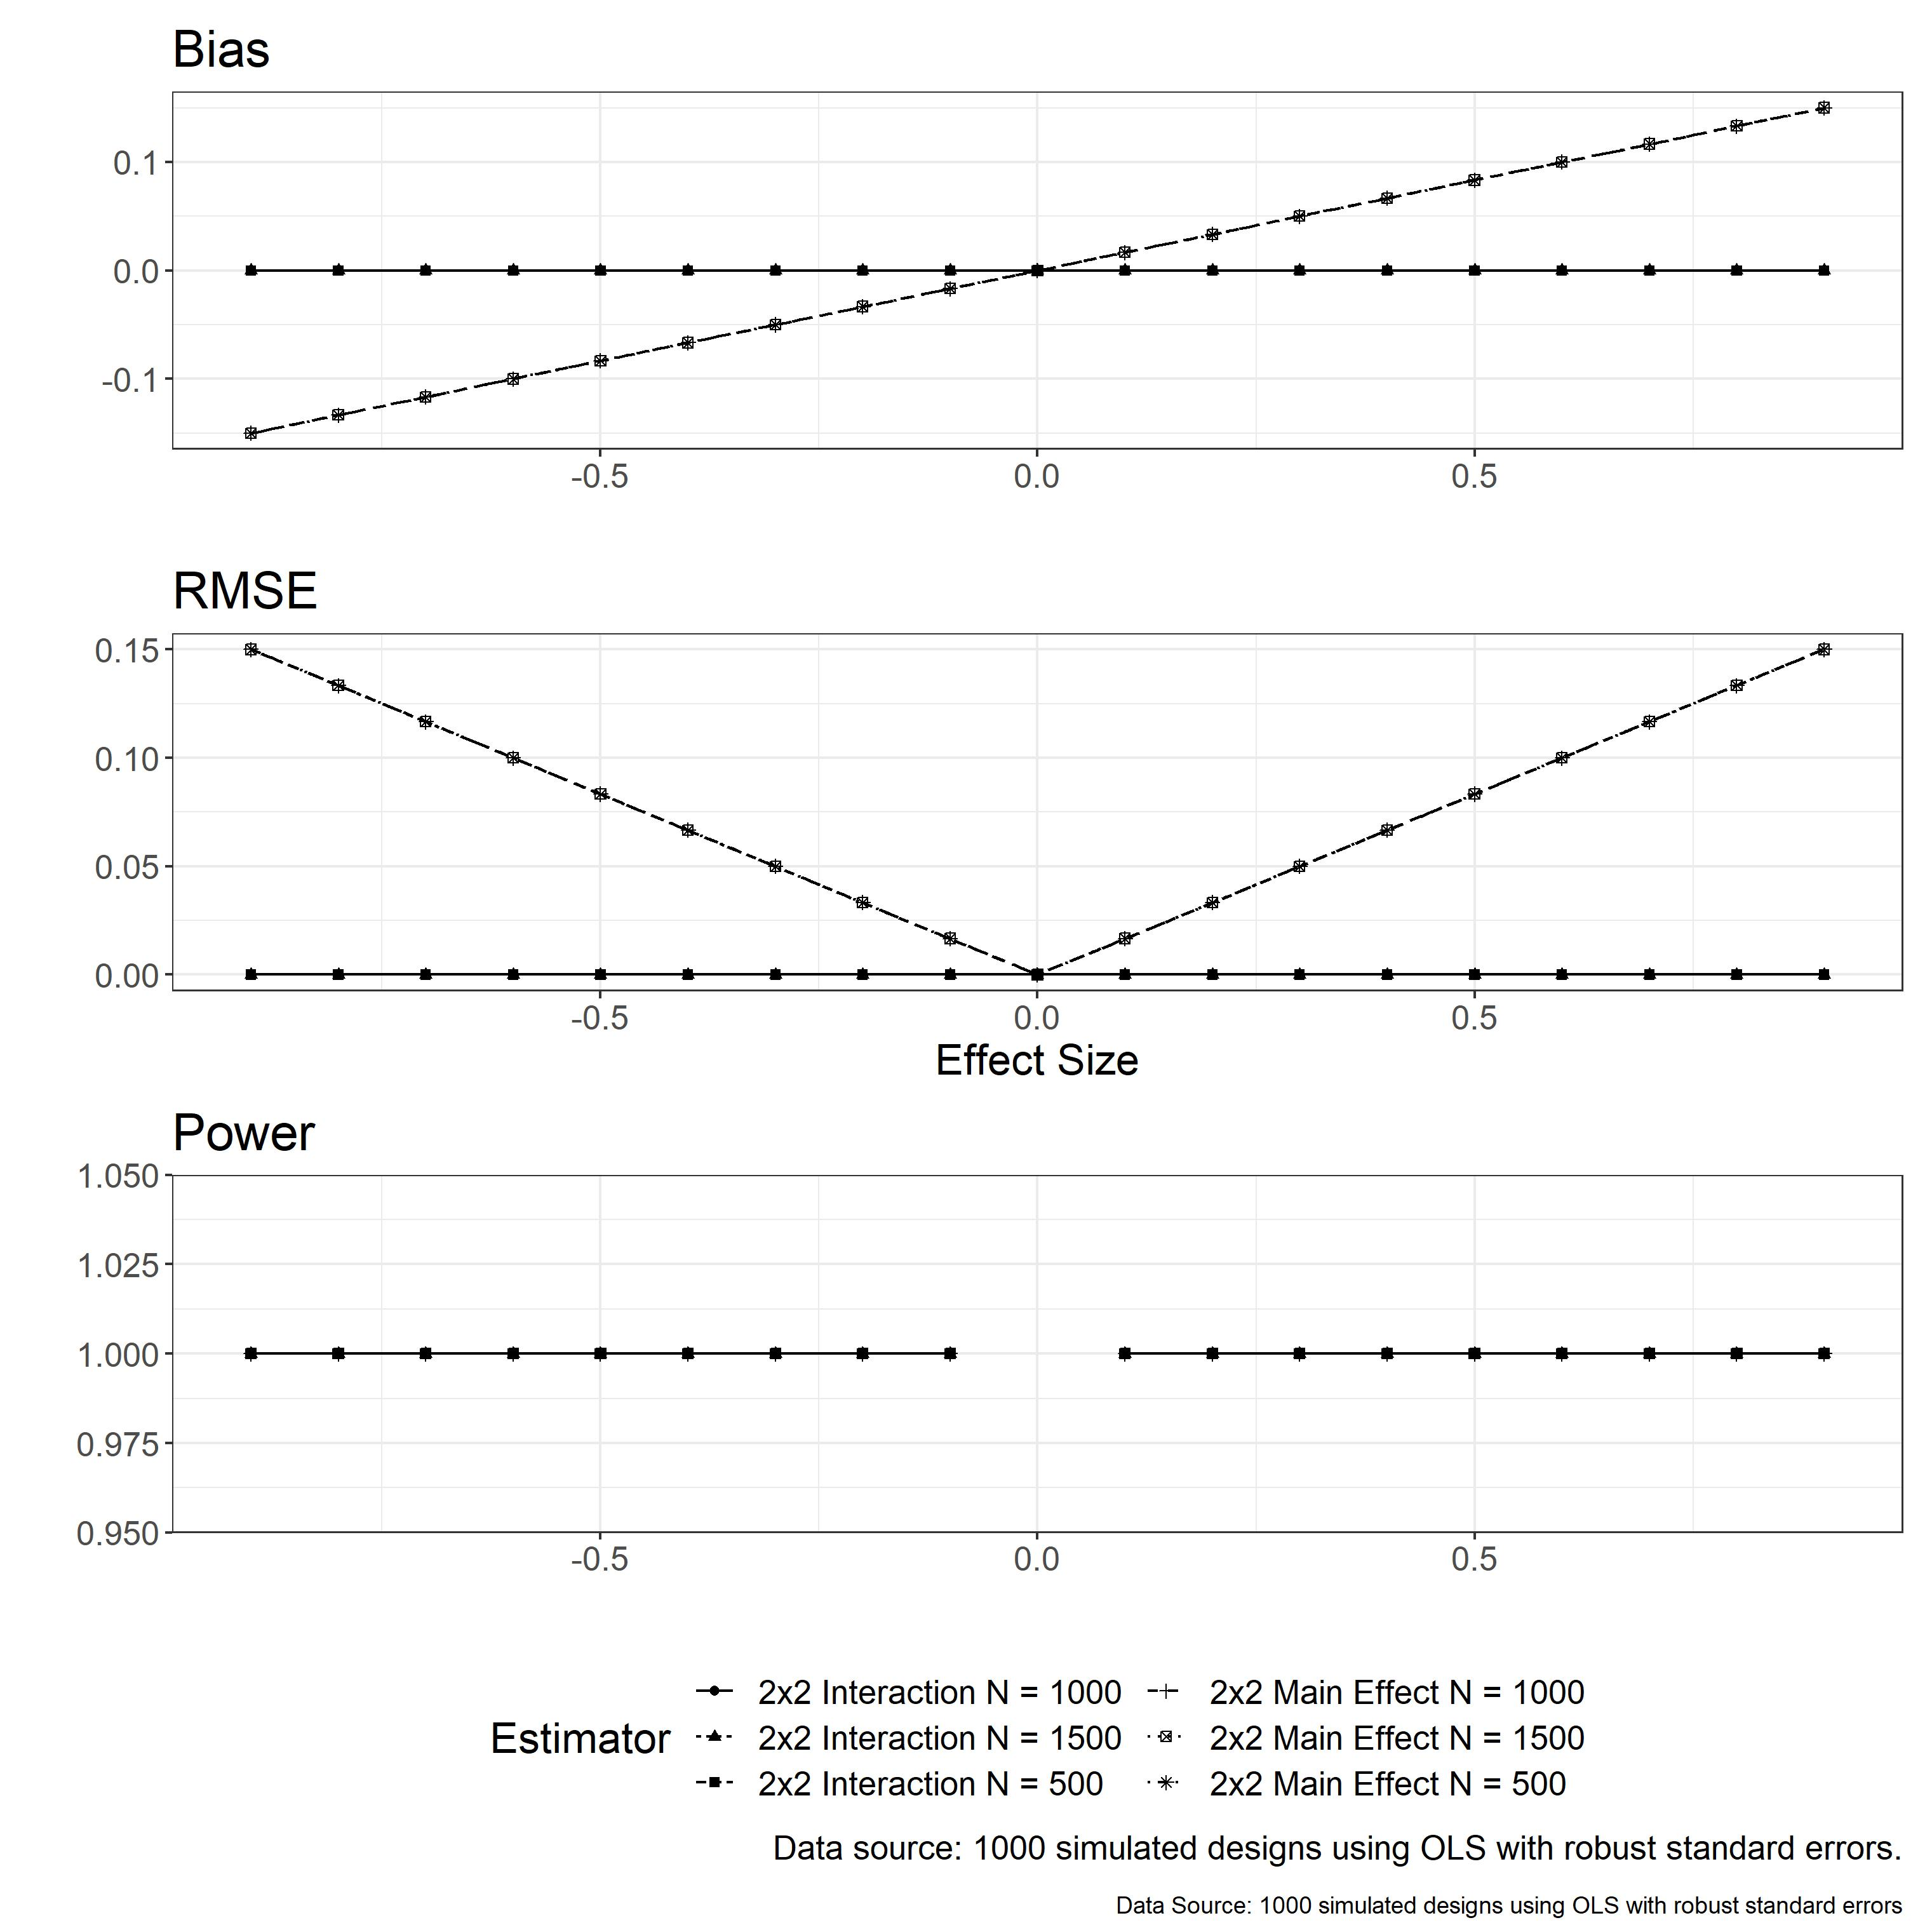
\includegraphics[width = 175mm]{../../figures/study_1_diagnoses.jpeg}
%     \caption{Comparison of Study 1 estimators}
%     \label{fig:study1}
%\end{figure}

%The results from the simulation suggest that the performance of both models are quite similar. While the interaction term for the block design shows lower statistical power in the plot, the scale of the plot ranges from $\tilde 0.99$ to $1$. To gain interpretive leverage of the news consumption variable as causal, I want to ensure that back-door paths are closed. Therefore, I elect to use a block design as randomization into treatment is determined within the block rather than across all levels of news consumption.

\subsection{Study 2}
To test $H_2$, the outcome of interest is the degree to which respondents punish or reward out-partisan elites who engage in differencing behavior with the individual's co-partisan representatives. Likewise, the hypothesis expects that individuals reward co-partisan elites who engage in this same differencing behavior with the individual's out-partisan representatives. From the discussion above, the data generating process under randomization is expected to be:
\begin{equation}
\begin{aligned}
\text{Punish}_i = \text{treatment}_i + \text{partisan congruence}_i + \\
     \text{treatment}_i \times \text{partisan congruence}_i + \\ 
     \epsilon_i
\end{aligned}
\end{equation}


\subsection{Study 3}
To test $H_3$, the outcome of interest is degree of polarization, measured as the difference between reported feeling thermometer scores between the two parties, as determined by whether one is primed, by recieving the treatment, or not. The data generating process under randomization is expected to be:
\begin{equation}
\begin{aligned}
\Delta \text{PID Feeling Termometers}_i = \text{treatment}_i + \text{partisan congruence}_i + \\
     \text{treatment}_i \times \text{partisan congruence}_i + \\ 
     \epsilon_i
\end{aligned}
\end{equation}

The expected data generating processes suggests that I should use a 2x2 factorial design. The 2x2 factorial design randomly assigns participants into a congruent partisan differencing, incongruent partisan differencing, a congruent partisan no differencing, or an incongruent no differencing condition. This randomization should close backdoor paths that may threaten my ability to calculate the causal effects of the treatments. For participants who are assigned into either of the differencing conditions, $\text{treatment}$ is coded as $1$ and $0$ if in one of the two no differencing conditions. If they are assigned into either of the two partisan congruence conditions, $\text{partisan congruence}$ is coded as $1$ if assigned into a condition where the politician is a co-partisan with the subject and $0$ if the politician is an out-partisan. I will then use linear regression where I examine the main effects of the differencing treatment and partisan congruence along with an interaction term for the two conditions. Specifically, my simulation fits a linear regression with robust standard errors. So long as one's model is properly specified, I should expect no differences between classical and robust standard errors. To be sure whether they are different, I will use the General Information Matrix test proposed by \citet{king_roberts_2015_pa}. 

Rather than use a 2x2 factorial design, I could instead use a 4-arm design. However, to fit the linear regression model, I would create two indicators for the differencing and partisan congruence treatment assignment and include main and interaction effects. Therefore, I do not believe there would be meaningful differences between the two studies. What I do consider, however, as interaction terms often require more degrees of freedom to achieve similar levels of statistical power, is whether I expect that my particular design and target sample size have sufficient power.

\begin{figure}[H]
     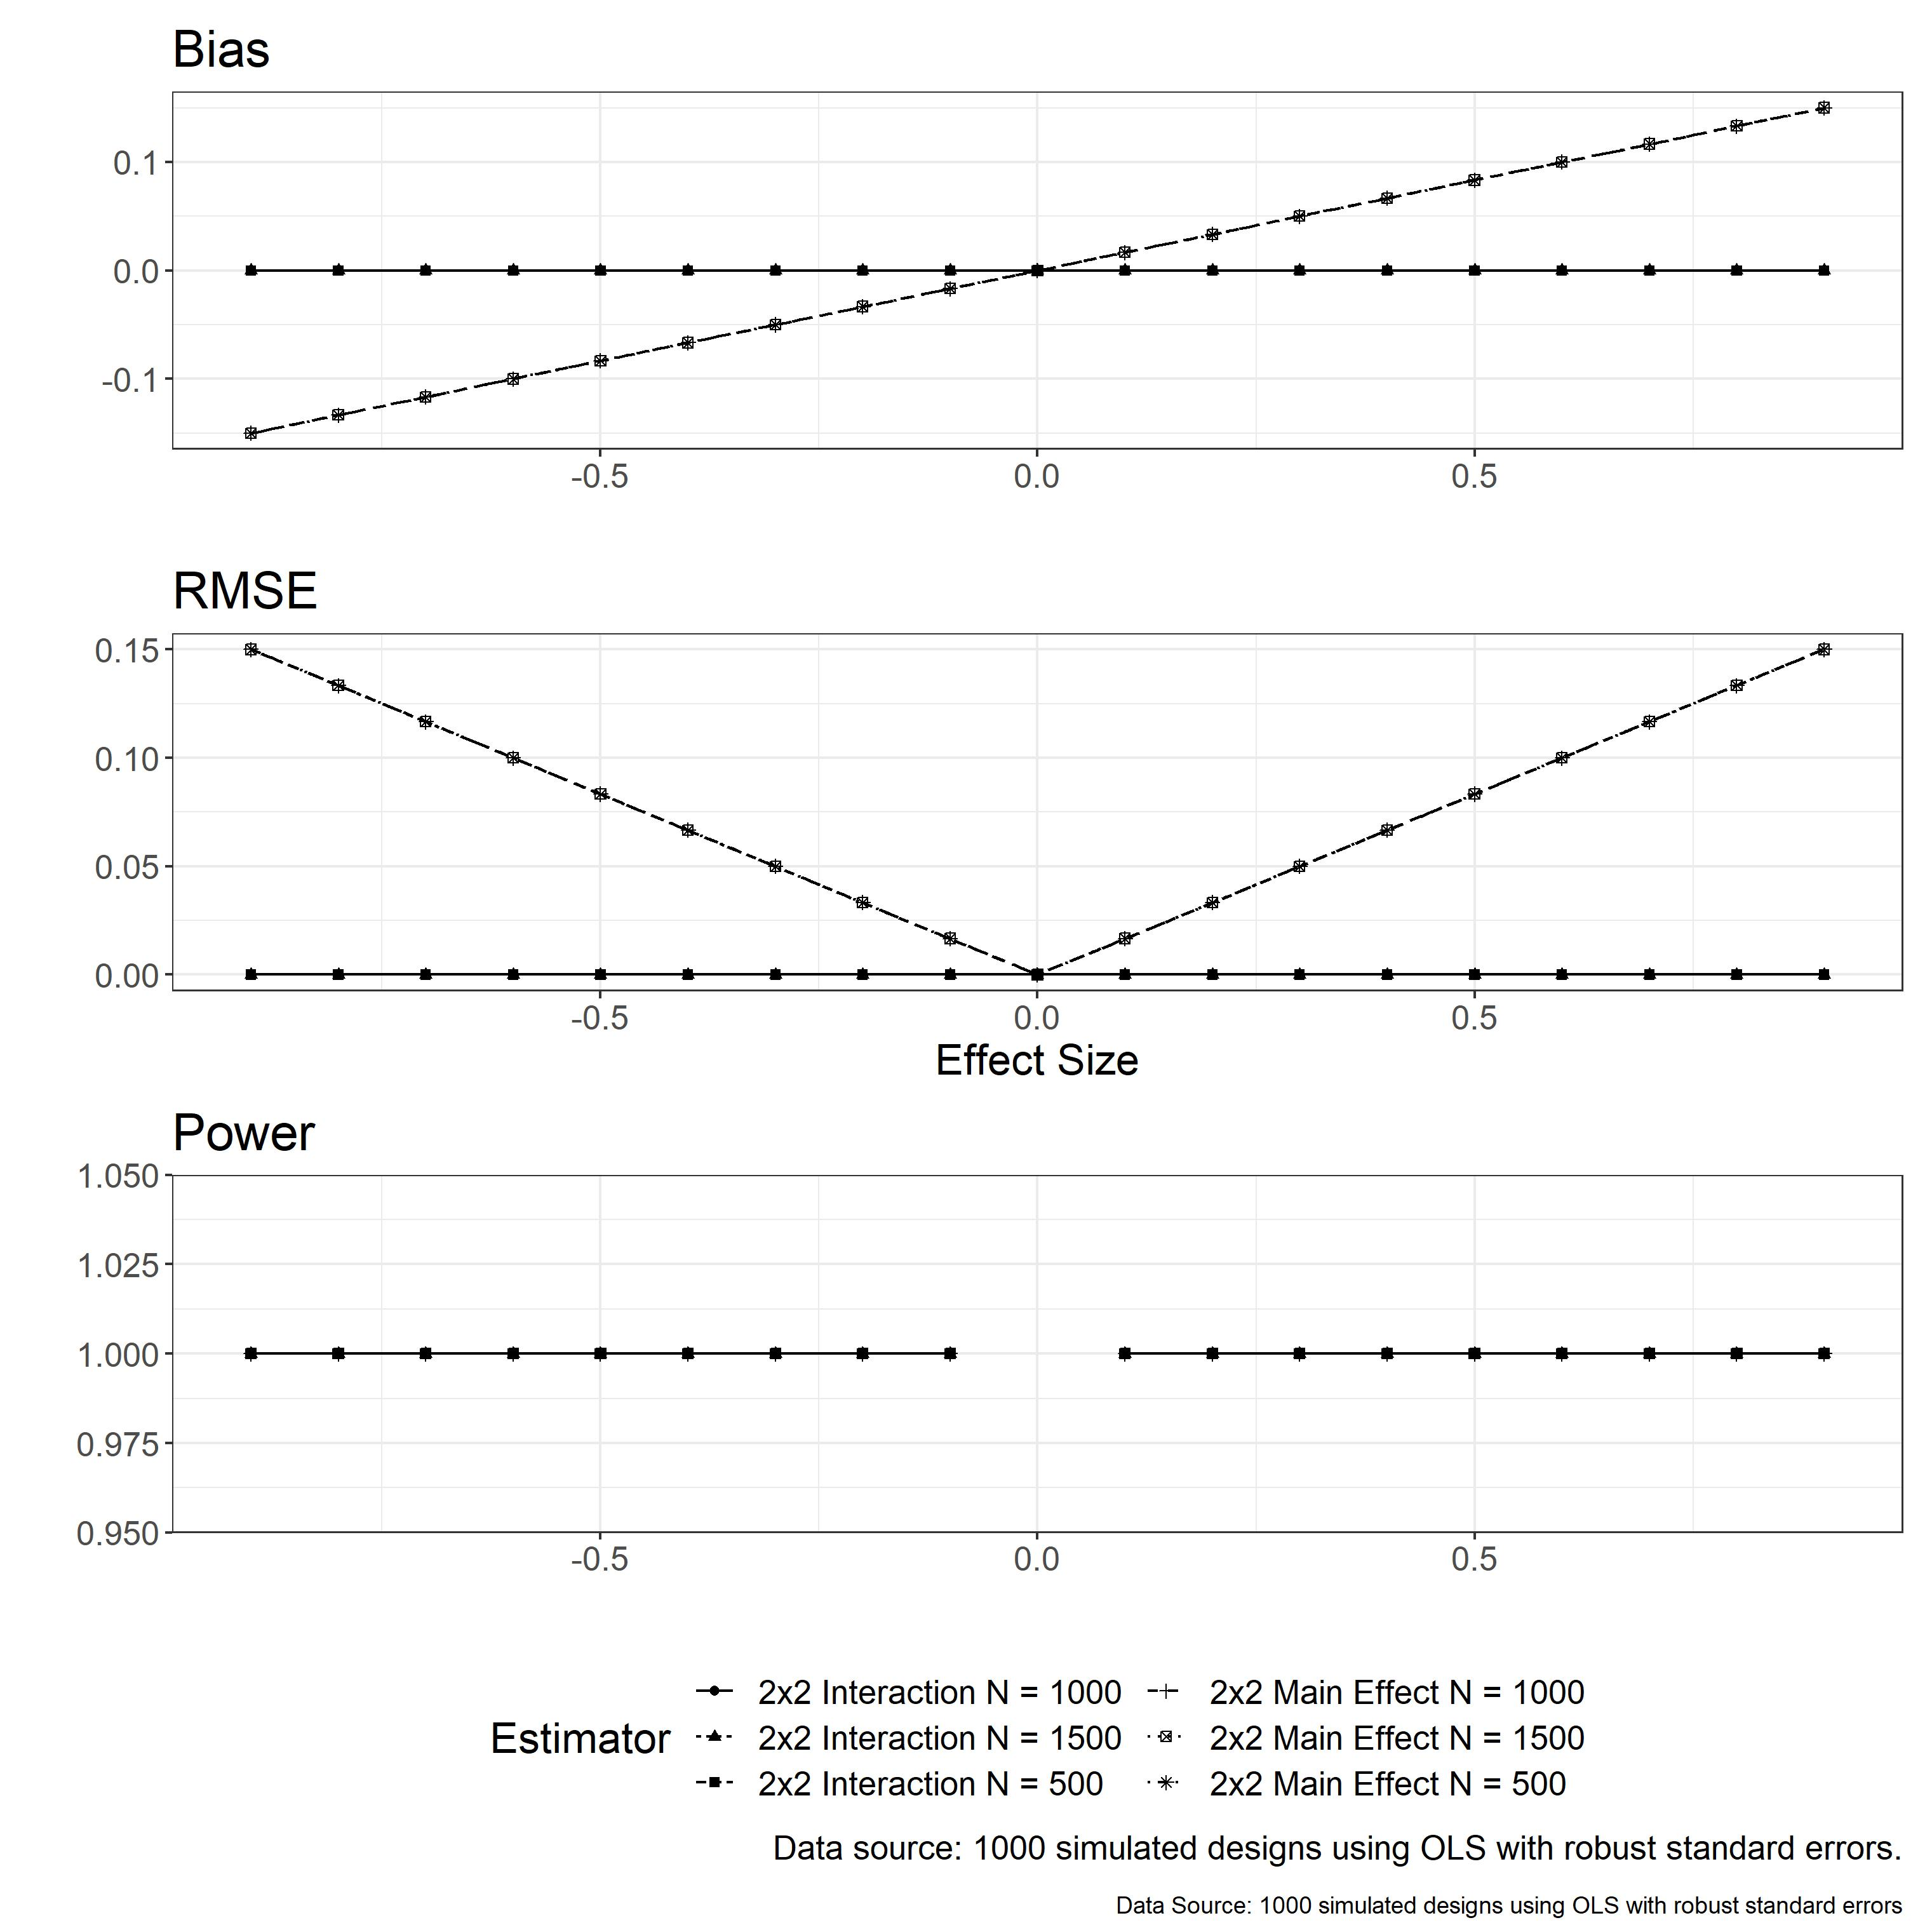
\includegraphics[width = 175mm]{../../figures/study_1_diagnoses.jpeg}
     \caption{Comparison of Study 1 estimators}
     \label{fig:study}
\end{figure}

As including interaction terms from a factorial design in regression require a larger sample for similar levels of statistical power, I use the \verb|declareDesign| package \citep{blair_et-al_2022_fabricatr} to examine the performance of the design along with the intended estimator at varying sample sizes from 500 total participants (n = 125 in each condition) to 1500 total participants (n = 375 in each condition). 

I define effect sizes that range from $-0.9$ and $0.9$. I also specify target sample sizes as $500$, $1000$, and $1500$. The simulated study relies on linear regression with robust standard errors. I choose robust standard errors rather than classical standard errors as \citet{king_roberts_2015_pa} demonstrate their use for identifying model misspecifications. In cases that model misspecification has been resolved, these standard errors should be equivalent to those of classical standard errors. I then simulate $1000$ studies with each of these features. \Cref{fig:study} presents the Bias, RMSE, and Power from the estimates. The results suggest that I should have sufficient power and little to no bias with a sample of $1000$ participants and this holds across the range of my effect sizes.

\section{Proposed protocol}

After providing their informed consent, participants will be asked to to provide a number of demographic questions including their partisan identification. Participants will then be randomly assigned into one of four conditions based on the combination of the focus being on partisan-congruent or partisan-incongruent members of congress and a treatment that highlights difference and elite polarization or one that emphasizes bi-partisanship and unity. 

\begin{quote}
	Congress introduced a new bill today. The bill \textbf{[disliked by Republicans/disliked by Democrats/disliked by many/disliked by many]} is meant to address funding concerns for high-use interstate highways. In reference to the bill, \textbf{[Republican Leadership/Democratic Leadership/a Republican-lead bipartisan coalition/a Democrat-lead bipartisan coalition]} expressed their feelings indicating that they felt this bill was not important. During the floor vote \textbf{[Republicans spoke at length about the Democrats' desire to slow Congress down with "pointless bills"/Democrats spoke at length about the Republicans' desire to slow Congress down with "pointless bills"/prominent Republicans representing a bipartisan coalition spoke at length about their belief that there are more pressing concerns/prominent Democrats representing a bipartisan coalition spoke at length about their belief that there are more pressing concerns]}. Afterwards on the floor, \textbf{[Republicans were huddled talking about how to make sure it doesn't come back up for a vote next session/Democrats were huddled talking about how to make sure it doesn't come back up for a vote next session/Republicans joined Democratic colleagues in a huddle talking about strategies to make sure it doesn't come back up for a vote next session/Democrats joined Republican colleagues in a huddle talking about strategies to make sure it doesn't come back up for a vote next session]}. That afternoon, when speaking to the press, \textbf{[Republican leaders talked about how Democrats don't care about the well-being of the country and are becoming more out-of-step with Americans/Democratic leaders talked about how Republicans don't care about the well-being of the country and are becoming more out-of-step with Americans/Republican leaders talked about how great it is to make sure everything is just right to make the bill work for Americans/Democratic leaders talked about how great it is to make sure everything is just right to make the bill work for Americans]}.
\end{quote}

Immediately following the treatment, participants will be presented with an attention check on a separate page asking them ``In the brief news report that you just read, what was the bill about?''. Subjects who are unable to answer the question or do so incorrectly will be excluded from later analyses. 

Once they have responded to the attention check, I will then ask the subjects the three questiosn that will be the dependent variables in the three studies:
     \begin{enumerate}
          \item Which statement do you think characterize the behavior of the politicians covered in the brief report the best:
          \begin{itemize}
               \item Unified
               \item Normal
               \item Divided
          \end{itemize}
          \item Do you think the party leaders should be:
          \begin{itemize}
               \item Rewarded by others in the party for how they handeled the situation
               \item Others in the party shouldn't do anything as a result of how they handeled the situation
               \item Punished by others in the party for how they handeled the situation
          \end{itemize}
          \item On a scale of $0-100$ where $0$ represents ``Cold'' and $100$ represents ``Very Warm'', how do you feel about:
          \begin{itemize}
               \item Republicans
               \item Democrats
          \end{itemize}
     \end{enumerate}

\newpage
\bibliographystyle{apsr}
\bibliography{C:/Users/damon/Dropbox/bibliographies/representation/polarization.bib,C:/Users/damon/Dropbox/bibliographies/representation/partisanship.bib,C:/Users/damon/Dropbox/bibliographies/representation/identity.bib,C:/Users/damon/Dropbox/bibliographies/representation/attitudes.bib,C:/Users/damon/Dropbox/bibliographies/representation/elite_cue_taking.bib,C:/Users/damon/Dropbox/bibliographies/institutions/institutional_theories/congress/parties.bib,C:/Users/damon/Dropbox/bibliographies/methods/experiments.bib,C:/Users/damon/Dropbox/bibliographies/methods/glm_mle.bib,C:/Users/damon/Dropbox/bibliographies/methods/software.bib,C:/Users/damon/Dropbox/bibliographies/institutions/institutional_theories/policy_outcomes.bib}
\end{document}